\paragraph{QuizziPedia::Front-End::Directives::FooterDirective}
\begin{figure} [ht]
	\centering
	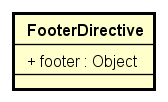
\includegraphics[scale=0.80]{UML/Classi/Front-End/QuizziPedia_Front-end_FooterDirective.png}
	\caption{QuizziPedia::Front-End::Directives:FooterDirective}
\end{figure} \FloatBarrier
\begin{itemize}
	\item \textbf{Descrizione}: \textit{directive\ped{G}} contenente i componenti grafici del footer dell'applicazione;
	\item \textbf{Utilizzo}: premette di visualizzare le informazioni contenenti nel footer in ogni pagina dell'applicazione;
	\item \textbf{Relazioni con altre classi}:
	\begin{itemize}
		\item \textbf{IN \texttt{Index}}: contenitore generale dell'applicazione.
	\end{itemize}
	\item \textbf{Attributi}:
	\begin{itemize}
		\item \texttt{+ footer: Object} \\ Oggetto contenente le informazioni presenti nel footer.
	\end{itemize}
\end{itemize}